\chapter{人-机器人交互研究理论基础}

\section{闭环人机交互过程的不确定性分析}
人-机器人交互问题可以被认为是一个协商性的协同控制过程,在此过程中使用者与系统共同沟通意图。因此,每一种类型的交互过程都有某种形式的不确定性,通常在大多研究中的目标都是引入更多的传感器信息去试图设计一个更精准的方法去推断使用者的意图从而忽略其中不确定因素的存在。在本文,我们认为在人机交互过程中的不确定性本身是一种信息,应该需要被正确地认识和对待,并且必须表示和处理所存在的不确定性,而不是盲目地过滤或忽略掉它。人机交互过程的不确定性来源繁杂,涉及人的行为、决策、机器的感知和决策、协同任务的目标设定以及交互方式等多个方面,大致有以下几种类型:(1)人的行为不确定性:人的行为受到情绪、健康状况、认知能力等因素的影响,导致其在与机器进行协同工作时的表现不确定。(2)人类决策的不确定性:人类在面临选择时,由于信息不完全、知识有限、环境复杂等因素导致无法确定最佳选择的情况。(3)机器的感知不确定性:机器在与人进行协同工作时,需要对人的行为和环境进行感知和理解。然而,由于感知技术的限制,机器对于人的行为和环境的理解往往存在不确定性。(3)机器决策的不确定性:由于机器学习算法的限制或数据的不完整性、不准确性等因素导致机器无法确定最佳决策的情况。(4)协同任务的目标不确定性:协同任务的目标通常由人和机器共同制定,但由于人和机器的意见、知识和经验的不同,目标的制定存在一定的不确定性。(5)交互方式的不确定性:人机协同中的交互方式往往是通过交互界面、语言或手势等方式进行的,但这些交互方式存在一定的不确定性。

已有研究对人-机器人交互在多智能体框架中进行建模分析,其中机器人和人都被视为智能代理\cite{liuDesigningRobotBehavior}。因此,本章首先从具有较好理论研究基础的智能机器人行为设计出发,对机器智能的设计实现过程进行分析。为了尽可能地适用于更多的交互场景和传感器使用,在此基础上,通过将人类交互行为视为一个连续的闭环控制过程,本章进一步分析了交互过程中的不确定性因素来源。

\subsection{机器人行为建模}
为了生成所期望的机器人行为,从优化控制的角度需要从三个方面进行设计\cite{liuDesigningRobotBehavior}:(1)以内部成本的形式向机器人提供有关任务要求的正确知识,并且向机器人提供关于外部环境的内部动力学模型;(2)设计一个的正确的决策模型,使得机器人可以将内部的知识表征转化为想要的动作;(3)设计一个学习方法来更新机器人的内部知识和决策模型,使得机器人可以在不同的环境中的动作决策具有泛化性。在图\ref{fig:2-1}中给出了机器人行为建模设计的框图,其中知识表征、决策模型以及学习算法为三个主要部分。机器人通过从人机混合的外部环境中获取环境数据$s$并根据其决策模型$d$和内部的损失函数以及内部的动力学模型约束$M$产生动作$a$。由于环境改变或所设计的知识表征无法满足当前场景的处理,因此需要学习来自环境的数据以更新内部的知识表征和决策模型。

机器人的行为系统开发主要分为三个阶段:设计阶段、训练阶段和执行阶段,其中设计和训练通常是离线完成的,而执行是在线进行的。在训练阶段,机器人可以从人类经验或来自人类的示教演示中学习知识。其中从人类的示教中学到的知识与人类设计的知识之间的区别在于,前者仅需要提供数据而不需要人类对知识的表征有数学或定量的表示。因为在大多数情况下,知识是抽象的且对人类来说是不直观的,我们往往无法显式地描述一个技能或知识,因此难以获得可靠的知识数学表征(例如,人类直接绘制出一个轨迹比设计出该轨迹的数学函数表达式更容易)。在执行阶段,机器人执行特定任务并与人类互动,能够通过在线学习更新其知识或逻辑。然而,受计算能力限制,在线学习通常只适用于参数的小规模自适应。如果从零开始学习一项新技能,这通常需在训练阶段通过离线学习完成。训练和执行阶段可以在同一学习系统内迭代进行。在外部环境或任务相对简单的情况下,机器人可直接从设计到执行阶段,无需经过训练。

\begin{figure}[h]
    \centering
    \includegraphics[width=0.6\textwidth]{2-fig-1.pdf}
    \caption{机器人行为建模设计结构框图}
    \label{fig:2-1}
\end{figure}
知识表征是一个机器人行为系统的核心,但是现在对于知识中由人类设计与后天学习各自所占的比重应当是多少仍然需要被进一步研究。其中内部成本是一个取决于机器人的状态和动作的函数,可分为静态成本和动态成本。静态成本是对当前状态和动作的一个函数。动态成本是一个进入未来的轨迹上的一个函数,它是沿着轨迹的所有静态成本的折扣累加。在内部模型的建立上,对于人-机器人混合的系统来说,由于机器人的刚体模型往往可以通过欧拉法或牛顿法直接建立,通常可以认为是已知的。因此在该类交互系统中人类的行为需要被建模、学习和预测\cite{liuDesigningRobotBehavior,araiAssessmentOperatorStress2010,xinxuHumanBehaviorUnderstanding2010}。其中有三种模型可以用来描述人类的行为:(1)反应模型,通过使用确定性的状态空间描述一个人的动态模型,其输入是影响行为的识别特征。(2)理性模型,其中人类的决策过程可以被视为一个最优控制器,其成本函数取决于人类对应的行为和机器人的行为的认知,并根据观测来推理最佳行为。(3)贝叶斯模型,人类被视为一个存在不确定性的随机决策智能体,即人类的行动遵循一个以机器人的行为为条件的概率分布。

而行为系统中的另外两个组件,决策模型和学习过程的本质是一种算法,因此通常是由人类进行设计的。决策模型的设计通常由三种方式,其中前两种方法是基于模型的,需要给出显式的$J$和$M$:(1)在设计阶段,明确地求解以$M$为动力学约束的优化控制问题$d(s)=\min_a J(a,s)$进而得到一个精确的策略,由于内部代价是非凸的,所以决策函数$d$可能是不连续的;(2)在执行阶段在线求解优化控制问题,由于$J$的非凸性,在线计算的控制输入$u$可能只是一个局部最优;(3)在训练阶段使用无模型的参数函数(例如神经网络)来近似该策略。综合来看,决策模型的设计通常由以下四类:

\begin{itemize}
\item 由设计者指定内部成本和内部模型以及显式的决策函数表达,并明确地解决优化问题,不需要任何学习过程。代表性的方法是:(1)经典控制方法;(2)马尔可夫决策过程(MDP);(3)经典模型预测控制(MPC)方法。
\item 由设计者指定内部成本以及显式的决策函数表达,基于学习对内部模型进行辨识。代表性的方法是:(1)经典的自适应控制;(2)自适应MPC控制器。该类型方法的优点是,它可以对时变的外部环境进行处理,特别适用于人在环中的场景。
\item 由设计师明确设计决策算法和相应的学习方法。知识在训练阶段通过试错或专家演示来获得的。代表性的方法是:(1)基于模型的强化学习;(2)逆强化学习,如学徒学习。这种方法的优点是,在设计阶段不再需要对任务和环境进行数学建模。
\item 由设计者明确地设计学习方法,并使用一个参数函数(例如神经网络)来近似决策模型。机器人将在训练阶段获得关于环境的知识(例如,网络中的参数),因此在这类方法中知识不是明确地学习的,而是隐式地编码在网络中。代表性的方法是:(1)无模型强化学习,如深度强化学习;(2)模仿学习。该方法通常适用于任务和环境极其难以建模,或者状态空间太大以及对实时计算要求较高的场景中。
\end{itemize}

机器人的行为的学习过程根据观测的数据更新知识和决策模型。学习可以在离线(在培训阶段)和在线(在执行阶段)中进行。在人-机器人交互中,机器智能的离线学习过程通常建立模型用于对人类行为进行描述或分类识别。另一方面,在线学习能够使离线学习的模型适应于人类的在线时变行为。
\subsection{闭环人机交互过程}
人类作为高级别的智能体,其决策过程也可以通过类似于机器人行为系统建模的方式进行分析。不同于机器智能的行为可以被设计,人类智能通常是固有的,因此在一个人-机器人交互系统中我们仅仅能够通过对人类动作这种可观测的状态对其内部状态、模型、意图等进行估计。人机交互是一种对于人类动作信息的放大器,其中交互的质量决定了``放大的比率''\cite{williamsonContinuousUncertainInteraction2006}。一个人机交互接口通过某种形式的交互模式在用户和系统之间关于潜在信息的状态进行通信。从这个角度来看,人类使用人机交互接口操控外部设备的过程可以被认为是一个连续的闭环控制系统,其通过感知输入、显示和推理机制,不断地解释来自传感器的输出来推断用户的意图等内部潜在信息,并将结果通过视觉、听觉或触觉等方式反馈给用户形成闭环。因此,一个交互方式的交互质量可以被视为用户使用该设备引导系统走向预期目标的成本。人机交互接口的最终功能是以用户所花费的最小的努力最优地确定用户的意图。如果交互者能够在消耗更少能量的同时正确地指定它们的意图,那么可以认为一个交互接口比另一个交互接口更好。从信息论的角度来看,交互成本可以通过交互接口通信一比特的信息所耗费的能量所表征。如果在一组潜在的变化中,通信每一个比特的成本被最小化,那么一个人机交互接口的设计就可以被认为是``好的''。

从贝叶斯的角度来看,任何关于这个世界的知识在某种程度上都是不确定的,并且在一个系统中的每一个关于状态的表示都是不精确的。概率论为以理性的方式处理这些不确定性提供了一套有效的工具。例如,人机交互系统中的所有使用的传感器都有一定的噪声,因此人类交互动作输入的真实状态永远无法准确地知道。更普遍的不确定性来自交互的潜在意图变量和推断模型之间的不匹配。例如来自任何一组传感器的时间序列都可以证明用户的意图,虽然更准确的传感或更长期的测量可以累积更多的``证据''用于推断意图,但它们永远不能消除所有的不确定性。因此一个``好的''的交互系统应当使用控制回路来减少交互过程中的不确定性,相反一个``坏的''的系统往往放大了其中的不确定性。因此,为了保证人-机器人交互的安全性和效率,要考虑整个交互作用系统的不确定性,而不仅仅是其每个组成部分的不确定性。

人机交互中的不确定性具有多种来源。其中一些是物理上的、硬件上的限制,如电气(热)噪声、传感器错误校准、测量不确定性等。其他的存在于建模和计算中,例如由于从样本不足产生的分布中进行蒙特卡罗抽样产生的不确定性、理想的人类内部模型与实际模型之间的不匹配产生的认知不确定性等。图\ref{fig:2-2}给出了人机交互闭环控制回路存在的一些不确定性来源。

\begin{figure}[h]
    \centering
    \includegraphics[width=1\textwidth]{2-fig-2.pdf}
    \caption{闭环人机交互过程的不稳定性来源}
    \label{fig:2-2}
\end{figure}

\begin{itemize}
\item 观测不确定性:在$t$时刻,人类通过视觉、听觉、嗅觉、触觉以及本体感觉等感知系统对外部环境状态进行观测。然而,在一个交互系统中,我们往往不能为用户提供关于环境状态的全部反馈(例如在大多数的应用中系统仅提供了视觉反馈)。或者用户由于能力有限或感知能力缺失(如失明、脊髓损伤导致的触觉以及本体感丧失)仅能对部分的环境状态进行观测,进而由于信息不完整、不准确导致的观测不确定性。关于观测不确定性可以使用部分可观马尔科夫决策过程(POMDP)进行研究,相关的研究可以在工作\cite{torretresolsPOMDPbasedControlHybrid2022,youngPOMDPbasedStatisticalSpoken2012,zhengPOMDPModelLearning2018a}中找到。
\item 认知不确定性:在人类获得对于外部环境状态$s_t$的观测$o_t$后,由于对于真实世界模型的理解存在偏差等原因,人对外部环境的认知和预测可能存在不确定性和模糊性。这通常表现为使用者对于交互界面的工作逻辑不清晰导致的在使用交互设备无法清晰表达需求和意图;此外由于使用者对于机器的功能和特性的了解不够准确,可能会对机器的能力产生过高的或过低的期望,导致对机器的输出和反应产生困惑。这种不确定性体现在用户关于外部环境的知识存在偏差,具体表现为带有偏见的内部损失函数$J$以及不同于真实环境动态模型的内部模型$M$。与机器人行为建模类似,人类动作决策也可以被看作一个潜在的以内部模型$M$为约束的最优化问题$d(o_t)=\min_{a_t} J(a_t,o_t)$,因此不准确的认知会导致所做出的动作是次优的。关于认知不确定性矫正在人机交互中的研究可以在工作\cite{gongWhatItYou2020,golubLearningInternalDynamics,raffertyInferringLearnersKnowledge,reddyWhereYouThink2018,javdaniSharedAutonomyHindsight2018}中找到。
\item 动作不确定性:解决最优化决策问题后的输出是一个具有物理意义的动作$a_t$,例如外骨骼设备操控中的肢体的运动、手势交互中的手掌运动、鼠标的移动等等。动作的不确定性是指在人类在执行动作过程中出现的非预期的、随机的、无意识的微小波动或变化。这些噪声可能来自多个方面,包括生理、神经控制、环境等。预期的和产生的人体运动之间的偏差已经在神经科学以及运动科学等领域被广泛研究\cite{vanbeersRoleExecutionNoise2004,faisalNoiseNervousSystem2008,churchlandCentralSourceMovement2006},对于需要辅助机器人进行交互帮助的运动受损的人来说,固有的身体限制会增加意外动作偏离预期动作的可能性,从而导致不必要的机器人行为。关于人机交互过程动作不确定性的研究可以在工作\cite{gopinathCustomizedHandlingUnintended2021,jainProbabilisticHumanIntent2020}中找到。
\item 测量不确定性:人机交互接口通过不同类型的传感器对人所发起的动作进行测量,每一种测量方法都具有不同的信息容量、噪声特性、延迟、频率响应特性。常见的传感器噪声有非线性误差、迟滞误差、重复性误差、漂移等,此外温度、湿度、压力、振动等环境因素可能影响传感器的性能和精度,以及由于各种难以预测和控制的因素引起的随机误差从而导致测量结果的不确定性。为了降低传感器测量不确定性可以通过选择高性能传感器、进行环境变化补偿以及使用适当的信号处理技术和滤波器,以减小随机误差和噪声。
\item 计算不确定性:由于通过人机交互界面采集得到的传感器数据一般需要使用一个映射函数$f(m)$将获取的传感信息解码为人类潜在的交互命令$u_t$,在感知数据是大规模或多源的情况下会由于计算资源的限制导致不确定性。例如计算数值计算溢出、数值离散化精度限制以及由于时间限制导致的计算结果与精确结果之间存在的差异。计算不确定性可以通过使用性能更好的计算设备或优化算法减少。
\end{itemize}

来自交互接口的传感器数据处理和解码主要旨在建立一个从观测数据到期望输出的映射函数$f(m_t)$。为此,研究进一步采用了概率图工具对该闭环交互过程进行了分析,可将其建模为一个部分观测的马尔科夫决策过程(POMDP)。图\ref{3-fig-6}给出了从$t-1$到$t+1$时刻的人机交互过程的概率图模型。其中${g_t}$表示在外部环境中用户意图实现达成的目标,${s_t} \in {\text{S}}$是外部环境的在$t$时刻的状态(可用于表示本工作中光标或轮椅的状态)。${o_t}$是用户对环境的观测信息,其包括视觉、听觉、触觉、嗅觉以及对于前一时刻动作${a_{t - 1}}$的本体感觉反馈。根据当前状态${s_t}$和目标${g_t}$,以及当前对于环境的观测的信念,使用者根据内部的决策模型执行最优动作${a_t} \in \Theta $并收到奖励$R$。由于人机交互为一个人类贯序决策过程,在本工作中人类肩部的动作空间$\Theta $是高维度且连续的,因此不能用有限数量的离散量表示。因此,所设计开发的体-机交互界面可以被视为一种对于人类动作的量化表征工具,它将不可直接定义的人类物理动作${a_t}$通过观测和映射函数量化为有意义的低维命令${u_t}$。最后,${u_t}$通过环境的状态转移方程$T({s_{t+1}}|{s_{t}},{u_{t}})$进而改变外部环境的状态实现对设备的操控。

\begin{figure}[htb]
    \centering
    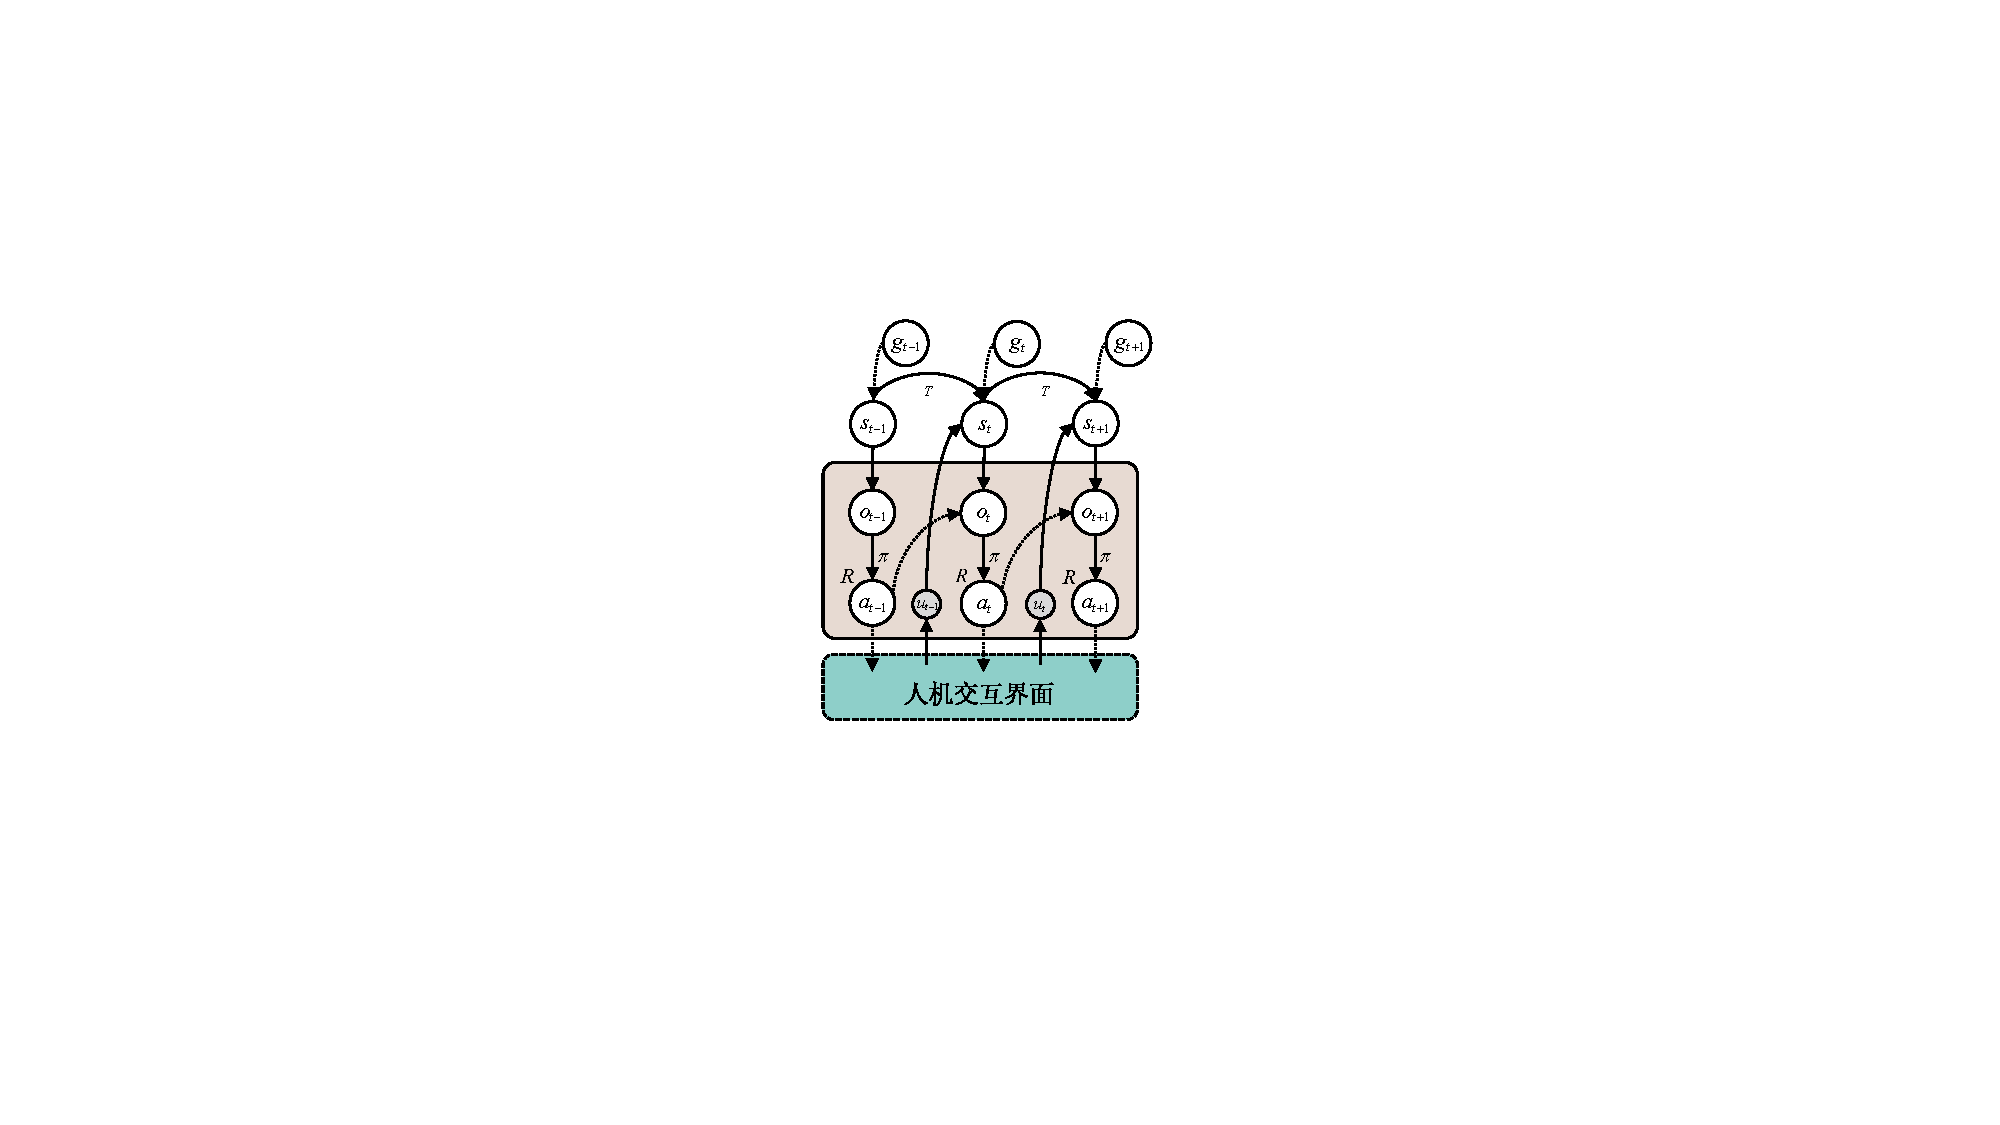
\includegraphics[width=0.3\textwidth]{3-Fig-6.pdf}
    \caption{闭环人机交互过程的概率图模型}
    \label{3-fig-6}
\end{figure} 

\section{人机共享自主}
完全自主的机器人能够在无需任何人类干预的情况下,通过感知、规划和行动来执行任务。尽管近年来自动化领域的研究取得了巨大进步,但我们仍然远远无法为机器人提供完全自主的能力,使其能够在非结构化环境中应对不可预测的事件或意外情况。由于具有更好的情境意识、逻辑和解决问题的能力,目前由人类操作员操作或监督机器人仍存在于大多数机器人应用中。传统的人-机器人交互模式的架构分为三类:(1)直接控制,系统中没有智能或自主性,机器人的所有自由度都由用户通过人机交互接口直接控制;(2)监控控制,用户命令和反馈发生在更高的层次,连接更松散,机器人必须依赖更强的局部自治来完善和执行任务;(3)共享控制,综合了机器人由直接用户命令和自主组合控制的所有中间级别。人机共享自主是指人类与机器之间建立一种共同的决策和行动框架,使得双方能够相互理解、协作和互补,以实现共同的目标。在这种关系中,人类和机器不仅仅是简单的工具或执行者,而是彼此平等地参与到决策和执行过程中,共同承担责任和权利。这种共享自主的模式旨在充分发挥人类和机器各自的优势,实现更高效、更智能的决策和行动,并最大程度地满足用户的需求和期望\cite{selvaggioAutonomyPhysicalHumanRobot2021a}。目前,在人机混合应用中共享控制方法已经在大量的半自动化的机器人中得到了应用,例如遥操作机械臂、手术机器人等。随着近些年来感知、建模以及识别技术的不断进步,共享自主在共享控制的基础上进一步扩展了原有方法的能力,其中在共享自主中一个人机混合系统可以通过以下动态方程描述:
\begin{equation}
    \begin{aligned}
    & \dot{x}(t)=g(x(t), u(t)) \\
    & u(t)=h_\theta\left(u_h(t), u_a(t) ; \theta(t)\right),
    \end{aligned}
    \label{eq:2-1}
\end{equation}
其中,$x$是机器人/环境状态,$u$是来自交互设备的控制输入。一个线性或非线性的仲裁函数$h_θ$结合/调制来自机器智能的控制$u_a$和人工输入$u_h$。仲裁函数$h_θ$通过调制两个输入$u_a$和$u_h$来决定机器人系统的自主水平。在这里,参数$θ$模拟了机器人对人类和/或由仲裁功能用来调节两个输入的环境的理解。例如,$θ$一般会包含有关人类动作/意图或任务完成状态的信息。共享自主系统一般基于环境参数$θ$来自适应调整人类和自主控制输入的权重。相反,在传统的共享控制系统中,仲裁函数中的环境参数$θ$一般是人为设定的固定值,因此$h_θ$可以简化为$h(u_h,u_a)$,即它不依赖于人类/自主控制输入以外的外部环境变量。
\begin{equation}
    h\left(u_h, u_a\right)=\alpha u_h+(1-\alpha) u_a
    \label{eq:2-2}
\end{equation}
其中,$α∈[0,1]$是在人类交互输入和机器自主控制器之间分配控制权限的权重。在共享控制中,权重$α$一般是由人类专家设计的,并且可以通过手动修改调整。当$α$被自动调优时,例如,通过对人类行为的推断或对人类输入的置信度的量化表征,其可以定义为共享自主系统。

传统共享控制可以提供对人类操作运动命令的校正或实现对子任务的控制,人类和机器人之间共享的自主性量,要么是静态的,要么是由人类手动调整的。目前在多自由度协作机械臂遥操作\cite{kronhardtUnderstandingSharedControl2023},手术机器人\cite{zhangHumanRobotSharedControl2022}以及电动轮椅控制\cite{qinanliDynamicSharedControl2011}等场景得到了应用。共享自主则通过对环境的感知,更加适应人和机器人之间的物理交互具有不断进化的性质,这使得人与机器人之间的交互更接近于人与人之间的互动。目前共享自主系统的动态自主性主要基于外部信息来调节,通常可以从人类状态或环境状态中获取。从技术实现角度来看,基于人类状态感知的共享自主系统一般从以下三个层面进行自主权动态调节:
\begin{enumerate}
\item 人类意图识别:意图识别一般从概率上对人类意图推断出人类在执行的任务,共享自主系统基于意图的概率计算出机器人必须采取什么行动,调节机器人的自主性和/或提供辅助。例如,针对遥操作机器人的交互问题,研究\cite{jainProbabilisticHumanIntent2020}基于一个递归贝叶斯滤波器和多模态的交互观测数据来进行人类的操控目标推断,并基于目标估计的不确定性度量实现了系统的自主级别调整。基于一个线性仲裁函数,研究\cite{gopinathHumanintheLoopOptimizationShared2017}通过估计人对于辅助机械臂目标的置信度量来确定自主控制器和人之间的权重。此外,博弈论方法也可以用于构建共享自主框架,基于闭环人机交互过程并假设人类通过优化目标函数进行决策,研究\cite{liFrameworkHumanRobot2016,liContinuousRoleAdaptation2015}从交互反馈误差推断人类潜在意图,以确定人机协同装配任务中变阻抗控制器的参数
\item 人类肌肉活动:通过测量肌肉活动并动态调节共享自主权的系统通常以最小化该肌肉活动为优化目标。例如,针对人类与协作机器人完成锯木头任务,在研究\cite{peternelAdaptationRobotPhysical2016}中实现了一个混合力/阻抗控制器,通过可穿戴的EMG传感器在执行任务时估计人体上肢肌肉活动,当其超过一个阈值时,机器人会使用学习到的操作技能来帮助人类减少肌肉疲劳。
\item 人类操作技能:通过区分用户的技能熟练水平来调整共享自主系统的辅助特性。例如,在研究\cite{enayatiSkillbasedHumanRobot2018}通过修改辅助机器人系统的行为,并通过防止对熟练用户的不必要的限制来增强用户体验。研究\cite{millikenModelingUserExpertise2017}基于POMDP用于表示远程移动机器人操控者的专业水平,并基于推断用户的专业水平和对环境状态的观测来实现用户输入与自主控制器的融合。
\end{enumerate}

此外,使用环境信息实现动态自主权调整是设计共享自主系统的另一种方式。目前,相关的研究主要通过从专家用户在执行某些任务时的示教行为数据模仿学习,并使用这些信息来帮助非专家用户完成类似的任务以提高交互效率来进行。例如,在遥操作任务中,将专家用户的操控轨迹与相应的环境信息编码到一些概率分布中,然后通过自适应控制器来确定系统的自主性\cite{abi-farrajLearningbasedSharedControl2017}。在远程执行的钉孔任务中,基于高斯混合模型从专家操作员的演示中提取信息,然后用于生成基于力的触觉引导轨迹,帮助非专家用户完成插入任务\cite{perez-del-pulgarUsingLearningDemonstration2016}。此外,在相关研究\cite{balachandranAdaptiveAuthorityAllocation2020a}中提出了一种处理目标遮挡的共享自主框架,基于自适应贝叶斯滤波器的目标测量不确定性,通过滤波器的协方差矩阵调节共享自主的权重。在设计共享自治系统时也可以综合使用人类和环境信息,但是如何正确地组合并确定从多个来源收集的信息的优先级目前还有待研究。

对于交互对象和任务本身以及任务执行环境的理解是实现共享自主系统中动态自主权调整的核心。在这里的``理解''不仅仅是一个对于环境态势或人类运动状态/意图的分类或识别任务,在算法实现层面上需要实现对运动技能的量化表征以及相关推理过程的置信度表征。因此,基于概率模型以及贝叶斯方法的算法设计框架在共享自主系统中被广泛采用。相较于统计模型,概率模型能够量化人机交互过程中的不确定性,并提供关于预测结果的置信区间或概率分布,此外贝叶斯方法能够在模型中传递不确定性,使得不确定性能够在整个推理过程中得到合理地传递和更新,为实现共享自主系统提供了可能。更重要的是,概率模型和贝叶斯方法更加适用于获取数据难度较大的物理人机交互领域,通过将先验知识或信念直接融入模型中,可以在获取少量数据的情况下实现意图推理或识别。

\section{运动技能模仿学习}
共享自主系统需要对人类或环境理解,相较于无监督学习,在人机交互应用中人类技能模仿学习作为一种监督学习方法可以使得机器智能更快地学习和掌握复杂的技能和知识,并且可以更好地适应复杂的环境和任务。例如在\ref{fig:2-2}所示的闭环人机交互过程中,通过获取环境数据$s$与交互接口对人类动作$a_t$的测量$m_t$或交互接口输出的命令$u_t$组成的数据对$[s,m_t]$或$[s,u_t]$,训练一个深度神经网络来模拟专家的行为,这种方法通常被称为行为克隆(Behavioral Cloning, BC)。此外,更深层次的模仿学习如逆强化学习(Inverse Reinforcement Learning, IRL),可以通过从专家的示教行为中学习其内部损失函数$J$和认知模型$M$,然后通过该模型来设计机器智能使其能够自主地模仿专家决策。然而,在辅助机器人的研究当中,需要完成的交互一般为连续的(例如机器人辅助关节运动),因此技能通常以轨迹的形式呈现。在实际应用中,我们仅能获取单个或少量的运动示教轨迹,因此需要运动技能轨迹模仿学习从中提取特征并泛化到不同的场景中。其不仅可以用于设计机器人的行为,更一般地可以作为一种手段用于表示交互过程中的人类行为以实现人机共享自主。

行为克隆和逆强化学习等模仿学习算法主要侧重于解决马尔科夫决策过程中的决策问题,其主要特点是需要与环境交互并且任意时刻的交互都会影响下一时刻。运动技能轨迹模仿学习则侧重于对于在一段时间内的人类连续动作$a_{1:T}$的理解和规划,其输入通常为时间或者其他无环境交互影响的状态\cite{HuangJiQiRenYunDongGuiJiDeMoFangXueXiZongShu}。机器人技能模仿学习的概念最早由美国南加州大学的Schaal等人\cite{schaalImitationLearningRoute1999}提出。此外,大量的实验证据表明生物系统能够将基本的运动单元进行组合和适应性调整,从而完成复杂任务,这一观点最终促成了运动基元理论的提出\cite{saverianoDynamicMovementPrimitives2023}。在后续研究中,Ijspeert等研究者\cite{ijspeertDynamicalMovementPrimitives2013,righettiDynamicHebbianLearning2006}根据弹簧阻尼模型,进一步提出了动态运动基元。这是一种“一次模仿学习(One-Shot Imitation Learning)”的方法,通过单一示范轨迹就能实现点到点或周期性运动的泛化。对于多条轨迹的学习,Paraschos及其团队提出了概率运动基元(Probabilistic Motion Primitive, ProMP),该方法通过最大似然估计来处理轨迹参数的概率分布,并依靠高斯条件概率运算来实现轨迹的泛化。此外,参数化的高斯混合模型\cite{paraschosProbabilisticMovementPrimitives2013}、隐马尔可夫模型\cite{rabinerIntroductionHiddenMarkov1986}以及基于核技巧的核化运动基元(Kernel Motion Primitive, KMP)\cite{huangKernelizedMovementPrimitives2019}都实现了人类运动时间序列的泛化学习。尽管不同的实现方法在收敛性以及输入输出方式上存在差异,作为元学习的一种,这些方法都对数据的依赖较小,目前在娱乐游戏、医疗机器人、自动驾驶以及人机交互中得到了广泛的应用。下面就本文中使用较多的动态运动基元DMP进行介绍,其根据应用的场景不同具有多种变体。

\subsection{离散动态运动基元}
离散动态运动基元通常描述点到点的运动轨迹,其特点是在运动开始和运动结束时的速度为零。动态运动基元源于生物系统的运动控制,可以被看作是一种稳定的非线性动力系统的严谨数学表述,其本质是一种从示教轨迹中学习位置$y$和速度$\dot{y}$到加速度$\ddot{y}$的映射函数。来自人类的示教运动轨迹通常是一个连续的时间序列,在算法运行的过程中通过假定已经观测到当前时刻$t$的轨迹位置和速度${y_t,\dot{y_t}}$已知,DMP通过将训练数据封装成一个线性二阶动力学模型(一个质量-弹簧-阻尼器系统)计算当前的期望加速度$\ddot{y_t}$,并由此获得下一个时刻的期望位置$y+\dot{y}\Delta t$和期望速度$\dot{y}+\ddot{y}\Delta t$\cite{HuangJiQiRenYunDongGuiJiDeMoFangXueXiZongShu}。给定一条长度为N的轨迹$\{ t_n,y,\dot{y},\ddot{y} \}_{n=1}^N$一个单自由度离散DMP由以下一组非线性微分方程定义:
\begin{equation}
    \dot{z}=\tau \alpha_z\left(\beta_z(g-y)-z\right)+f(x)
    \label{eq:2-3}
\end{equation}
\begin{equation}
    \dot{y}=\tau z 
    \label{eq:2-4}
\end{equation}
\begin{equation}
    \dot{x}=-\tau \alpha_x x
    \label{eq:2-5}
\end{equation}
其中$z$是一个辅助变量。$α_z>0$和$β_z>0$为常数分别用于表示刚度和阻尼系数,一般在应用中设置为$α_z=4β_z$$\tau$的比例可以保证系统稳定收敛,此外还可以在保持系统收敛性的同时,从训练数据中学习到增益$α_z$和$β_z$\cite{tanApplyingAdaptiveControlb}。$\tau$为轨迹的时间缩放系数,时间$t$以可微的相位变量$x$表示。在式\ref{eq:2-3}中的$g$表示轨迹的目标位置。$f(x)$为一个改变弹簧阻尼系统的外部强迫项,其被定义为由$N$个非线性径向基函数(RBF)的线性组合,使机器人能够跟踪从初始位置$y_0$到最终目标位置$g$的任何平滑轨迹,其定义如下:
\begin{equation}
    f(x)=\frac{\sum_{i=1}^N w_i \Psi_i(x)}{\sum_{i=1}^N \Psi_i(x)} x
    \label{eq:2-6}
\end{equation}
\begin{equation}
    \Psi_i(x)=\exp \left(-h_i\left(x-c_i\right)^2\right)
    \label{eq:2-7}
\end{equation}
其中,$c_i$是沿运动相位分布的高斯基函数的中心位置,其宽度为$h_i$。对于一个给定的基函数数量$N$,设$τ$等于所需运动的持续时间,则基函数的中心位置可以定义为$c_i=\exp \left(-\alpha_x i-1 / N-1\right)$,基函数宽度定义为$h_i=1 /\left(c_{i+1}-c_i\right)^2$。若轨迹是高自由度的,对于每个自由度的权重$w_i$应该从单独的训练数据中进行学习,以达到期望的行为轨迹。权重数量的选择应基于所需的轨迹分辨率,当需要更高分辨率轨迹的时候使用。对于一个具有多个自由度的行为系统,可以给予每一个自由度自己的动态系统如公式\ref{eq:2-3}和\ref{eq:2-4}来表示每个自由度的运动,但用公共相位\ref{eq:2-5}来同步各个自由度轨迹的迭代运行。

\subsection{节律动态运动基元}
当需要被DMP编码的运动遵某种节奏模式时,可以使用节律型DMP(也称周期DMP)进行处理。节律DMP在离散DMP的模型的基础上主要改变了相位变量。在节律DMP中重新定义的二阶系统的公式为:
\begin{equation}
    \dot{z}=\Omega(\alpha(\beta(g-y)-z)+f(\phi))
    \label{eq:2-8}
\end{equation}
\begin{equation}
    \dot{y}=\Omega z
    \label{eq:2-9}
\end{equation}
\begin{equation}
    \Omega \dot{\phi}=1
    \label{eq:2-10}
\end{equation}
其中不同于离散型DMP,在节律型DMP中与轨迹持续时间相关的时间常数被所编码轨迹的频率$\Omega$所取代。此外,节律型的DMP必须确保初始阶段$\Phi = 0$和最终阶段$\Phi = 2\pi$一致,以便在轨迹重复过程中实现平稳过渡。与离散DMP类似,节律型DMP同样也由$N$个RBF基函数定义,其唯一区别是基函数的中心位置是在0到$2\pi$的连续相位空间内均匀分布的,其表达式如下:
\begin{equation}
    f(\phi)=\frac{\sum_{i=1}^N \Psi_i(\phi) w_i r}{\sum_{i=1}^N \Psi_i(\phi)}
    \label{eq:2-11}
\end{equation}
\begin{equation}
    \Psi_i(\phi)=\exp \left(h\left(\cos \left(\phi-c_i\right)-1\right)\right)
    \label{eq:2-12}
\end{equation}
其中,权值沿相空间均匀分布,参数$r$用于调制周期信号的振幅。
\subsection{动态运动基元的学习}
DMP中用于的权重参数$w_i$是线性的,因此可以使用各种类型的监督学习框架来拟合$w_i$,此外如果只有来自成本函数的信息可用,许多其他优化算法也可以被使用。其中学习的过程分为两个阶段\cite{saverianoDynamicMovementPrimitives2023}:第一步是确定高级参数的取值,例如离散DMP中的目标位置g,初始位置$y_0$,时间常数$τ$,第二步为从示教轨迹中学习参数$w_i$。

对于离散DMP,参数$g$可以设置为示教轨迹结束时的位置,类似的初始状态$y_0$设置为轨迹开始的位置。在实际使用中,时间缩放系数$τ$设置为示教序列的持续时间,但是从记录的示教轨迹中提取$τ$需要一些额外的轨迹检测分割算法来确定运动的开始和结束位置\cite{tanApplyingAdaptiveControlb}。例如,可以采用轨迹最大速度的2\%作为分割阈值,$τ$可以选择为持续时间的1.05倍用于补偿由于阈值化而导致的轨迹开始和结束时的缺失。对于节律DMP,$g$是一个周期轨迹基准锚点,一般设置为所示教周期轨迹的中间位置,可用于调整周期信号的基准位置。此外,在节律DMP中的参数$\Omega$被一般并被设置为所演示的节奏运动的周期除以2π,在实际应用中,周期信号的频率信息需要被傅里叶分解等方法额外计算。由于离散DMP和节律DMP的二阶系统主要差别在于时间缩放系数$\tau = 1/\Omega$,因此在这里仅分析离散DMP的学习过程。当给定一个组演示轨迹及其关于时间的一阶导数和二阶导数$\{y_{demo},\dot{y}_{demo},\ddot{y}_{demo} \}$可以通过改写式\ref{eq:2-3}得到一个函数近似问题,其中强迫项$f$需要尽可能得逼近示教轨迹形状$f_{target}$:
\begin{equation}
    f_{target}=\tau^2 \ddot{y}_{demo}-\alpha_z\left(\beta_z\left(g-y_{demo}\right)-\tau \dot{y}_{demo}\right)
    \label{eq:2-13}
\end{equation}
学习的过程基于局部加权最小二乘法(LWR)进行\cite{schaalConstructiveIncrementalLearning1998},此外也可以使用混合模型或者高斯过程等其他的函数逼近器来进行。通过寻找外部强迫项$f$中每个核函数对应的$w_i$使得由下式定义的局部加权二次误差最小:
\begin{equation}
    J_i=\sum_{t=1}^P \Psi_i(t)\left(f_{\text {target }}(t)-w_i \xi(t)\right)^2
    \label{eq:2-14}
\end{equation}
其中,离散DMP的$ξ(t) = x(t)(g−y_0)$而节律型DMP的$ξ(t) = r$,计算该加权线性回归问题,有两种求解方法,当可以获得完备的示教数据时,使用离线学习方法获取权重$w_i$:
\begin{equation}
    w_i=\frac{\mathbf{s}^T \boldsymbol{\Gamma}_i \mathbf{f}_{\text {target }}}{\mathbf{s}^T \boldsymbol{\Gamma}_i \mathbf{s}}
    \label{eq:2-15}
\end{equation}
其中:
\begin{equation}
    \mathbf{s}=\left(\begin{array}{c}
    \xi(1) \\
    \xi(2) \\
    \ldots \\
    \xi(N)
    \end{array}\right) \quad \boldsymbol{\Gamma}_i=\left(\begin{array}{cccc}
    \Psi_i(1) & & & 0 \\
    & \Psi_i(2) & & \\
    & & \ldots & \\
    0 & & & \Psi_i(N)
    \end{array}\right) \quad \mathbf{f}_{\text {target }}=\left(\begin{array}{c}
    f_{\text {target }}(1) \\
    f_{\text {target }}(2) \\
    \ldots \\
    f_{\text {target }}(N)
    \end{array}\right)
    \label{eq:2-16}
\end{equation}
此外,也可以通过递归最小二乘法实现权重$w_i$的增量学习,利用期望的轨迹形状与当前学习到的形状之间的误差和遗忘因子λ,在每个时间步迭代更新权重:
\begin{equation}
    \begin{gathered}
    w_i(t)=w_i(t)+\Psi_i P_i\left(t\right) \xi(t) e\left(t\right), \\
    P_i\left(t_{J+1}\right)=\frac{1}{\lambda}\left(P_i\left(t\right)-\frac{P_i\left(t\right)^2 \xi(t)^2}{\frac{\lambda}{\Psi_i}+P_i\left(t\right) \xi(t)^2}\right)
    \end{gathered}
    \label{eq:2-17}
\end{equation}
其中,参数的初始值分别为$w_i(0)=0$和$P_i(0)=1$,遗忘因子决定了权重更新的速率,其中残差定义如下:
\begin{equation}
    e\left(t\right)=f_{target}\left(t\right)-w_i\left(t\right) \xi(t)
    \label{eq:2-18}
\end{equation}
\section{本章小结}
在本章节中,我们首先对机器人行为系统的建模过程进行了总结和分析,在此基础上从人类的视角进一步分析了闭环人机交互过程的整个流程以及其中存在的不确定性来源。此外,就处理人机交互过程中的不确定性问题,引入了共享自主的概念和相关应用方式,并对其相关背景进行了介绍。最后,针对在共享自主方法中的人类行为表示方法,探讨了运动基元的相关理论,并就动态运动基元这一典型代表展开了详细的分析和介绍。